\section{Methods} \label{ICRA:sec:methods}

\subsection{Adapting the Dynamics} \label{ICRA:sec:adaptation}

At a high level, our method minimizes prediction error on $\DST$ by dynamically weighing the training data $\dataset$ such that transitions that are likely to be in $\DST$ are given weights near 1 and transitions unlikely to be in $\DST$ are given weights near 0. Given a transition from our training data $\transition\in\dataset$, we cannot directly evaluate whether that transition is in $\DST$, since that would require knowing the true dynamics $\targetDynamics$. However, since the initial dynamics, denoted $\learnedDynamics_0$, is assumed to accurately fit the source dynamics, it is likely that transitions with low prediction error under the initial dynamics $\distf{\learnedDynamics_0(\state,\action)}{\state'\big} < \softFilteringThrehsold$ are in $\DST$. By training on transitions with initially low error, we expect the prediction error on other transitions which belong to $\DST$ to also decrease. This slowly brings more and more transitions to have prediction errors below $\softFilteringThrehsold$. On the other hand, the prediction error is unlikely to decrease for transitions not in $\DST$, because they are dissimilar to the transitions with low initial error. Thus, at each step $j$ of training, we assign each transition a weight as a function of the prediction error $||\pred{\state}'-\state'||^2$, and multiply this weight by the loss. The full loss is shown in Equation \eqref{ICRA:eq:adaptation_loss}.

\begin{equation}
    \label{ICRA:eq:adaptation_loss}
    \begin{split}
    \mathcal{L}_\dynamics &= \frac{1}{T}\sum_{t=1}^T\Big(\dynamicsErrort w^t\Big) \\
    w^t &= 1 - \sigma\big(\phi(\globalStep)(\dynamicsErrort - \softFilteringThrehsold)\big)
    \end{split}
\end{equation}

$\sigma$ is the sigmoid function. When $\globalStep$ is large, the boundary is almost hard, and transitions with error below $\softFilteringThrehsold$ have weight near 1 and transitions with error above have weight near 0. When $\globalStep$ is small, the boundary is soft, and the weights vary less. The term $\phi(\globalStep)$ controls the rate of change of hardness. We use $\phi(j)=0.5j$ in our experiments. We found that allowing the weighting to be soft during early training steps improves the stability in the case where few or no transitions have error below $\softFilteringThrehsold$ at the beginning of training. The parameter $\softFilteringThrehsold$ can be chosen based on either the maximum error that can be corrected by a low-level controller, or based on the distribution of error on a validation set from the source environment (e.g the 97th percentile).

\subsection{Online Learning}

\begin{figure}
    \centering
    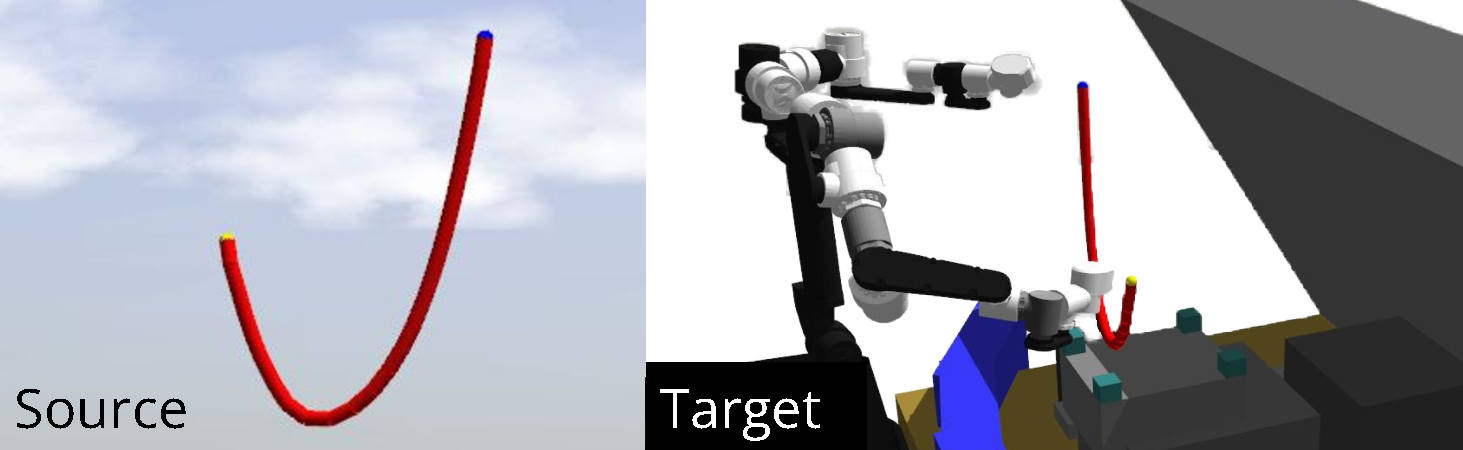
\includegraphics[width=\linewidth]{Chap4/images/sim_rope_envs.pdf}
    \caption{Source environment for bimanual rope manipulation (left) and simulated target environment (right) where there is a robot, obstacles, and the rope damping and stiffness are changed.}
    \label{ICRA:fig:sim_rope_envs}
\end{figure}

\begin{figure}
    \centering
    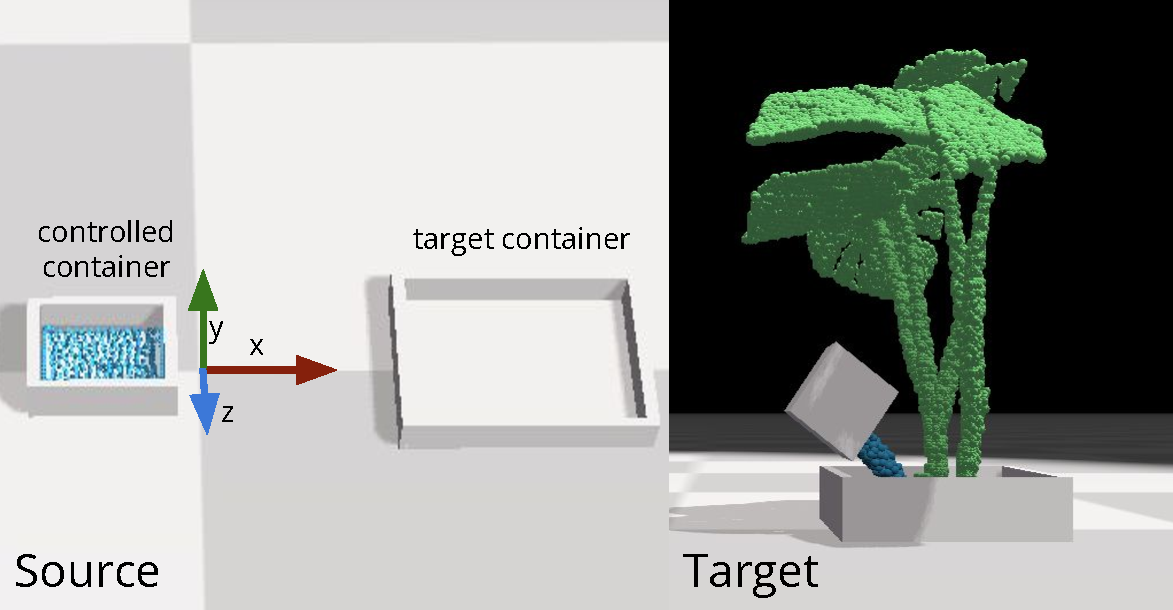
\includegraphics[width=0.7\linewidth]{Chap4/images/sim_water_envs.pdf}
    \caption{Source environment for plant watering (left) and target environment (right) where there is an additional plant, and the viscosity is tripled.}
    \label{ICRA:fig:waterscene}
\end{figure}

In this section, we describe how the proposed adaptation method can be combined with prior work on planning with unreliable dynamics to achieve data-efficient online adaptation of dynamics models. A block diagram of the full method, which we call \FOCUS{}, is shown in Figure \ref{ICRA:fig:diagram}. \FOCUS{} consists of an offline phase and an online phase. In the offline phase, we train a dynamics model using data from the source environment, which in our experiments is a simple simulation. We use random actions to collect a diverse set of data and standard techniques for training the neural network dynamics model \cite{UnreliableMitrano2021}.

In the online phase, we adapt the learned dynamics model to the target environment (e.g. the real world). This process alternates between (1) collecting new data in the target environment by planning and executing, (2) fine-tuning the dynamics, and (3) fine-tuning the model deviation estimator (MDE). We now explain the data collection and MDE fine-tuning steps.

\subsubsection{Planning and Execution for Data Collection}

We use a kinodynamic RRT planner where nodes are propagated using the learned dynamics model. Since the learned dynamics are adapting to only $\DST$ and are not accurate everywhere, we additionally constrain the planner to stay in $\DST$. Since $\DST$ is not known \textit{a priori}, we train another neural network, called a model deviation estimator (MDE)~\cite{MDEs22, UnreliableDale2019, UnreliableMitrano2021}, to predict the error of the dynamics model (more details in Section \ref{ICRA:sec:fine_tuning_mde}). In addition to producing more robust plans, planning with MDEs has the additional benefit of focusing data collection on $\DST$. By collecting more data where the source and target dynamics are close, a larger fraction of $\dataset$ is likely to be in $\DST$, and therefore the adaptation procedure has more data from which to learn.

We use the MDE in planning as a constraint checker. If the dynamics error predicted by the MDE is below a threshold $\dmax$, then we add it to the planning tree. We also randomly accept transitions with high predicted dynamics error with low probability (0.01), so that the planner will occasionally return paths with exploratory actions (we call these \textit{random-accepts}). These exploratory actions are essential for training the MDE, since they can correct over-estimation of model error from the MDE. The threshold $\dmax$ for allowable error is similar to $\softFilteringThrehsold$, but may be set higher or lower to control the exploration/exploitation tradeoff.

The robot uses the planner to attempt the task, and repeatedly plans and executes open-loop until a timeout or the goal is reached. If no plan is found that reaches the goal, the plan which gets closest to the goal is executed. This repeated planning and execution is called one episode. After some fixed number of episodes (e.g. 10) we fine tune the dynamics and the MDE using all data collected so far during the online phase.

\subsubsection{Fine-tune MDE}
\label{ICRA:sec:fine_tuning_mde}

The MDE is used to constrain planning to regions where the dynamics model is predicted to be accurate, which has two benefits. First, it helps bias data collection to contain transitions from $\DST$. Second, it makes reaching the goal more likely since it avoids plans that do not match to the true dynamics. The MDE $\pred{\mdeError}=\MDE(\env,\state,\action,\pred{\state}')$ is a convolutional neural network which takes as input the environment, state, action, and next predicted state, and predicts the error of the dynamics model $\pred{\mdeError}$. We represent the environment $\env$ as a voxelgrid of the scene. The ground truth error used for training is the error between the true observed state and the state predicted by the learned dynamics: $d=\distf{\pred{\state}'}{\state'}$. The loss function is shown in Equation \eqref{ICRA:eq:mde_loss}. Intuitively, the MDE should be easier to learn with fewer data than learning the dynamics accurately everywhere, since the MDE need only predict the magnitude of the error as opposed to the full state vector \cite{UnreliableMitrano2021}.

\begin{equation}
    \label{ICRA:eq:mde_loss}
    \mathcal{L}_{\MDE} = ||\pred{\mdeError} - \mdeError||^2e^{-{\kMDE \mdeError}}
\end{equation}

$\kMDE$ is a hyperparameter that reduces the need to predict high dynamics errors with high accuracy. We set $\kMDE=10$.
